\section{Python应用——傅里叶变换函数}

本章的一个重点是能够将一个时域图形变换成傅里叶频谱并分析。
本节编写Python傅里叶变换函数,并借助Python快捷地获得傅里叶变换。

本节要点:
\begin{itemize}
    \item 学会Python编写傅里叶变换函数;
    \item 掌握分析方法。
\end{itemize}

%============================================================
\subsection{Python傅里叶变换函数}

由于Python没有傅里叶变换的函数,Numpy和Scipy都只有FFT,所以编写一个傅里叶变换的函数。

根据傅里叶变换公式my\_fourier编写如下函数:
\[
X\left( \omega \right) =\int_{-\infty}^{+\infty}{x\left( t \right) e^{-i\omega t}dt}
\]

\begin{python}
def my_fourier(
        x:np.ndarray, t:np.ndarray,
        w_range:tuple=(-5*np.pi, 5*np.pi), num:int=500
        ) -> tuple:

    w = np.linspace(w_range[0], w_range[1], num+1)
    F = np.zeros_like(w, dtype=np.complex64)
    dt = t[1] - t[0]

    for n in range(F.size):
        F[n] = np.dot(x, np.exp(0-w[n]*t*1.0j)) * dt
        pass

    return (F, w)
\end{python}

参数:
\begin{itemize}
    \item x:np.ndarray类型,表示信号$x\left( t \right) $的值;
    \item t:np.ndarray类型,表示信号$x\left( t \right) $的时间;
    \item w\_range:元组类型,表示$\omega $的取值范围,需要原点对称;
    \item num:整数类型,表示$\omega $的离散个数,也即$\omega $的采样个数。
\end{itemize}

函数流程:
\begin{enumerate}
    \item 首先根据w\_range和num生成w,我们做的傅里叶变换就在这个范围内,也即$\omega $的采样点,0点对称;
    \item 初始化傅里叶离散点,注意F的类型是np.complex64;
    \item 循环,核心是做积分;
    \item 返回(F,w)表示$F\left( \omega \right) ,\omega $。
\end{enumerate}

%============================================================
\subsection{分析方法}

通常有一类问题是已知一个连续信号的时域波形图,要分析它的频域。借助我们的函数,一般步骤如下:
\begin{enumerate}
    \item 根据图形写出连续信号的时域函数;
    \item 用my\_fourier()求傅里叶变换;
    \item 用Matplotlib画出幅频图和相频图分析。
\end{enumerate}

%============================================================
\subsection{例}

\begin{example}
假设有信号$x\left( t \right) =p_2\left( t \right) $,用Python计算傅里叶变换,并作图。
\end{example}

用Python求解傅里叶变换并作图:

\begin{python}
t    = np.arange(-20, 20, 0.01)
x    = np.where(t<-1, 0, np.where(t>1, 0, 1))
X, w = my_fourier(x, t, w_range=(-6*np.pi, 6*np.pi), num=1000)

axs[0].plot(t, x)
plot_mag_phs(w, np.abs(X), np.angle(X, deg=True), ...)
\end{python}

\begin{figure}[h]
\centering
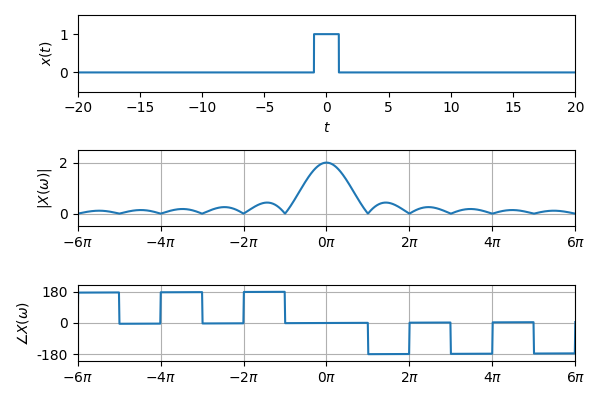
\includegraphics[height=5cm]{4.3.3-1.png}
\end{figure}

~

\begin{example}
设函数有如下图形,用Python分析傅里叶变换。
\begin{figure}[h]
\centering
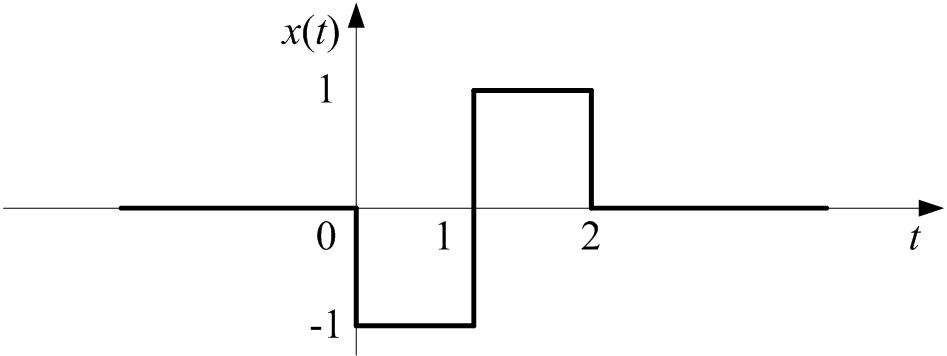
\includegraphics[height=2.5cm]{4.3.3-2.png}
\end{figure}
\end{example}

根据图形得到时域函数$x\left( t \right) =-u\left( t \right) +2u\left( t-1 \right) -u\left( t-2 \right) $,用Python求解傅里叶变换并作图:

\begin{python}
t    = np.arange(-20, 20, 0.01)
x    = np.where(t<0, 0, np.where(t<1, -1, np.where(t<2, 1, 0)))
X, w = my_fourier(x, t, w_range=(-6*np.pi, 6*np.pi))

axs[0].plot(t, x)
plot_mag_phs(w, np.abs(X), np.angle(X, deg=True), ...)
\end{python}

\begin{figure}[h]
\centering
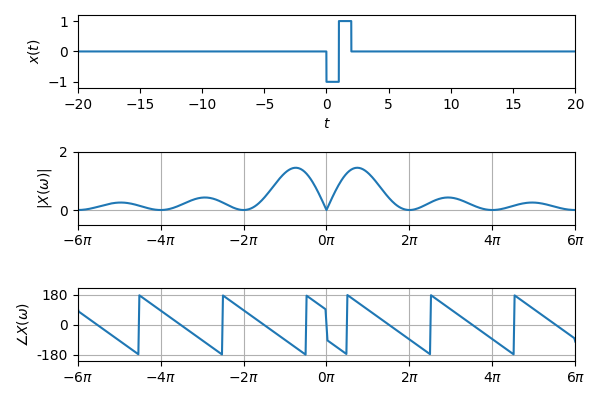
\includegraphics[height=5cm]{4.3.3-3.png}
\end{figure}

~

\begin{example}
设函数有如下图形,用Python分析傅里叶变换。
\begin{figure}[h]
\centering
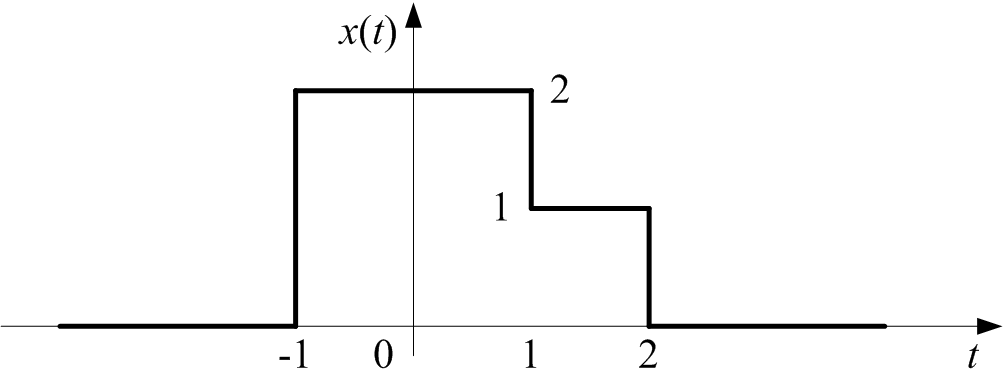
\includegraphics[height=2.5cm]{4.3.3-4.png}
\end{figure}
\end{example}

\begin{figure}[h]
\centering
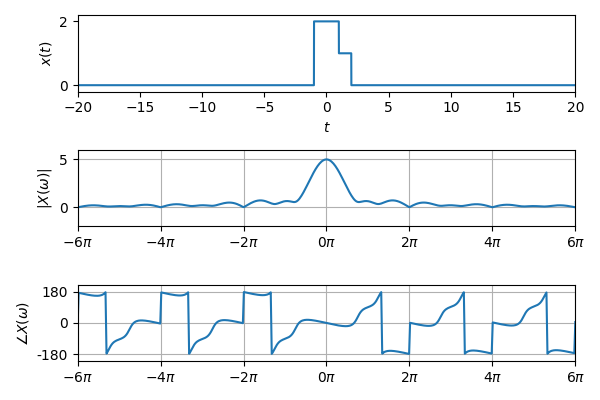
\includegraphics[height=5cm]{4.3.3-5.png}
\end{figure}

根据图形得到时域函数$x\left( t \right) =2u\left( t+1 \right) -u\left( t-1 \right) -u\left( t-2 \right) $,用Python求解傅里叶变换并作图:

\begin{python}
t    = np.arange(-20, 20, 0.01)
x    = np.where(t<-1, 0, np.where(t<1, 2, np.where(t<2, 1, 0)))
X, w = my_fourier(x, t, w_range=(-6*np.pi, 6*np.pi))

axs[0].plot(t, x)
plot_mag_phs(w, np.abs(X), np.angle(X, deg=True), ...)
\end{python}




